%!TEX root = ../main.tex

\chapter{Numerical Experiments}

In this section we describe the implementation of the algorithm. We also compare its performance with different alternative methods. Note that we focus on the univariate case. The implementation of our algorithm is the same in the multivariate setting.

\section{Introduction}
Before anything else, we remind the reader the problem setting and the estimator considered. We observe $n$ independent random vectors $\bX_1,\ldots,\bX_n\in\calX$ drawn from a probability distribution $P^*$ that admits a density function $f^*$. Given a family of mixture components $f_1,\ldots,f_K$, we assumed that this unknown density is well approximated by a convex combination $f_{\bpi}$ of these components
\begin{equation}
f_{\bpi}(\bx)=\sum_{j=1}^K\pi_j f_j(\bx), \quad \bpi \in \BB_+^K=\Big\{\bpi\in [0,1]^K: \sum_{j=1}^K\pi_j=1\Big\}.
\end{equation}
The component densities $\calF=\{f_j:j\in[K]\}$ are assumed to be given by previous experiments or expert knowledge. The problem of construction of this family is an open problem that we try to address in section ?\todos{en parler}. The objective of this chapter is to expose the algorithm implemented for the Maximum Likelihood Estimator (MLE), defined by
\begin{equation}
\label{MLE_2}
\hat\bpi \in \argmin_{\bpi\in \BB_+^K}\big\{-\frac{1}{n}\sum_{i=1}^n\log f_{\bpi}(\bX_i)\big\}.
\end{equation}
One can note that this problem is convex as the composition of $-\log$ and a linear function is convex. Furthermore, the feasible space is also convex. This problem can be solved via a Primal-Dual interior point method. But we will present a simpler approach based on an accelerated proximal gradient descent method.
\section{Implementation}
We can see that \cref{MLE_2} is equivalent to
\begin{equation}
\argmin_{\bpi\in\RR^K}\big\{-\frac{1}{n}\sum_{i=1}^n\log(f_{\bpi}(\bX_i))+\chi_{\BB_+^K}(\bpi))\big\},
\end{equation}
where $\chi_{\BB_+^K}$ is the indicator function
\begin{equation*}
    \chi_{\BB_+^K}(\bpi) =
    \begin{cases}
      0 & \text{if } \bpi\in \BB_+^K,\\
      \infty & \text{otherwise} .
    \end{cases}
\end{equation*}
This problem can be decomposed into 
\begin{equation}
\label{general_min_pb_fista}
    \min_{\bpi}\big\{f(\bpi)+g(\bpi)\big\},
\end{equation}
where $f(\bpi) =-\frac{1}{n}\sum_{i=1}^n\log(f_{\bpi}(\bX_i)$ and $g(\bpi)=\chi_{\BB_+^K}(\bpi)$. One can note that this problem is convex but not smooth since $f$ is differentiable but $g$ is not. One way to tackle this minimization is to consider the proximal operator
\begin{equation}
    \textnormal{prox}_{\lambda g}(\bpi) = \argmin_{u}\big\{g(u)+\frac{1}{2\lambda}\|u-\bpi\|^2_2\big\},
\end{equation}
where $\lambda > 0$ is a scale parameter for the function $g$. One can interpret $\textnormal{prox}_{\lambda f}(\bpi)$ as a point that compromises between minimizing $g$ and being near to $\bpi$. Note that in our context, $g(.)=\chi_{\BB_+^K}(.)$, therefore
\begin{align*}
    \textnormal{prox}_{\lambda g}(\bpi) &= \argmin_{u}\big\{\chi_{\BB_+^K}(u)+\frac{1}{2\lambda}\|u-\bpi\|^2_2\big\},\\
    &= \argmin_{u\in \BB_+^K}\big\{\|u-\bpi\|^2_2\big\},\\
    &= \bPi_{\BB_+^K}(\bpi)
\end{align*}
where $\bPi_{\BB_+^K}(\bpi)$ is the Euclidean projection of $\bpi$ into the set probability simplex. The reader can find in \citep{Parikh:2014:PA:2693612.2693613} a detailed study of proximal algorithms. A particularly interesting procedure for our problem is the proximal gradient method that solves \cref{general_min_pb_fista}. This method is iterative and the $(k+1)^{th}$ step is
\begin{equation}
    \bpi^{k+1} := \textnormal{prox}_{\lambda^k g}(\bpi^k-\lambda^k\nabla f(\bpi^k)),
\end{equation}
where $\lambda^k > 0$ is a step size. This step size can be found via a linesearch method \citep{Parikh:2014:PA:2693612.2693613}. However, if $\nabla f$ is $L$-Lipschitz, we can chose a fixed $\lambda^k\in (0,1/L)$. On this setting, one can show that this method converges with a rate of $\mathcal O(1/k)$. This rate is know to be sub-optimal. To circumvent this slow rate, accelerated versions of the proximal gradient method has been developed \citep{RePEc:cor:louvco:2007076}\citep{Beck:2009:FIS:1658360.1658364} that achieve optimal $\mathcal O(1/k^2)$ rate under the $L$-Lipshitz condition on $\nabla f$. These optimization methods relies on the proximal operator and Nesterov's Accelerated gradient method \citep{Nesterov:1983wy}. A version of this accelerated method is
\begin{equation*}
    \begin{cases}
    \xi^k &:= \bpi^k + \omega^k(\bpi^k-\bpi^{k-1}),\\
    \bpi^{k+1} &:= \textnormal{prox}_{\lambda^k g}(\xi^k-\lambda^k\nabla f(\xi^k)),
    \end{cases}
\end{equation*}
where $\omega^k$ is defined by
\begin{equation*}
    \begin{cases}
    \omega^1 &:= 1,   \\
    \omega^k &:= 2\frac{\omega^{k-1}-1}{1+\sqrt{1+(\omega^{k-1})^2}}.
    \end{cases}
\end{equation*}
This method is called Fast Iterative Shrinkage-Thresholding Algorithm (FISTA) from \citep{Beck:2009:FIS:1658360.1658364}. Our procedure is a special case of this algorithm that can be called 'Accelerated projected gradient descent' \todos{en italique} since the proximal is the projection into $\BB_+^K$. A procedure for the projection into the probability simplex can be found in \citep{Duchi:2008:EPL:1390156.1390191} and a simple proof in \citep{Wang13projectiononto}. The procedure for this projector is given in \cref{algo:proj_simplex.}. Finally, the complete procedure for our algorithm is given in \cref{fig:pi_fista}.\\ 
A nice property of this method is that it provides a sparse solution of this minimization problem which fits with our goal of selecting elements of the dictionary. General Primal-Dual interior points methods do not offer this feature.

\begin{figure}
\begin{center}
\mybox{
\begin{minipage}{0.85\linewidth}
\begin{algorithmic}%\SetAlgoLined\tt\SetLine
\small
\STATE {\bfseries Input: $\bpi\in\RR^p$.} 
\STATE {\bfseries Output:} The projection $\bpi^{proj}$ of $\bpi$ onto the probability simplex.
\STATE {\tt 1: Sort $\bpi$ into $\bu:\,u_1\geq u_2 \geq\dots\geq u_p$.}
\STATE {\tt 2: Find $\rho=\max \{1\leq j\leq p:\, u_j+\frac{1}{j}(1-\sum_{i=1}^j u_i) > 0\}$.}
\STATE {\tt 3: Define $\lambda = \frac{1}{\rho}(1-\sum_{i=1}^{\rho} u_i) > 0$.}
\STATE {\tt 4: Construct $\bpi^{proj}\,\textnormal{s.t.}\, \bpi^{proj}_i=\max\{\pi_i+\lambda,0\},\,i=1,\dots,p$.}
\end{algorithmic}
\end{minipage}}
   \caption{ Projection procedure onto the probability simplex}
   \label{algo:proj_simplex.}
\end{center}
\end{figure}

\begin{figure}
\begin{center}
\mybox{
\begin{minipage}{0.85\linewidth}
\begin{algorithmic}[1]%\SetAlgoLined\tt\SetLine
\small
\STATE {\bfseries Input:} A gradient step $\lambda$.
\STATE {\bfseries Output:} parameter estimate $\hat\bpi$.
\STATE {\tt 1: Initialize $t_0=1$ and $\bpi_0=(1/K,\dots,1/K)$,}
\FOR{$k\geq 0,$ until convergence occurs, }
\STATE {(a) $\bpi_k = \bPi_{\BB_+^K}\big( \xi_k - \lambda \nabla f_{\xi_k}(\xi_k)\big)$,}
\STATE {(b) $t_{k+1}= \frac{1+\sqrt{1+4t_k^2}}{2}$,}
\STATE {(c) $\xi_{k+1} = \bpi_k + \big(\frac{t_k-1}{t_{k+1}}\big)(\bpi_k-\bpi_{k-1})$.}
\ENDFOR.
\end{algorithmic}
\end{minipage}}
   \caption{Estimation of $\bpi$.}
   \label{fig:pi_fista}
\end{center}
\end{figure}

\section{Alternative methods considered}

\subsection{Adaptive Dantzig density estimation}

We will compare our method with the Adaptive Dantzig estimator in the density model which has been introduced in \cite{Bertin}. This method is similar to ours as it construct an estimator of the unknown density from a linear mixtures of functions taken from a dictionary. The key idea of this paper is to minimize the $\ell_1$-norm of the weight vector of the linear combination under an adaptive Dantzig constraint. This constraint comes from sharp concentration inequalities. We recall here some material about the Dantzig selector. It has been introduced by \cite{candes2007} in the linear regression model
\begin{equation}
	Y = A\lambda_0 + \epsilon
\end{equation}
where $Y\in \RR^n$, $A$ is a $n$ by $M$ matrix, $\epsilon \in \RR^n$ is the noise vector and $\lambda_0$ the unknown regression parameter to estimate. The Dantzig estimator is then defined by\todos{Définir $\ell_1$ et $\ell_{\infty}$}
\begin{equation}
	\hat\lambda^D = \argmin{\lambda \in \RR^M} \|\lambda \|_1 \quad \text{subject to} \quad \| A^T(A\lambda-Y)\|_{\infty} \leq \eta.
\end{equation}
where $\eta$ is the regularization parameter. \cite{bickel2009} considered the non-parametric regression framework
\begin{equation}
		Y_i = f(x_i) + e_i, \quad i=1,\dots,n
\end{equation}
where $f$ is an unknown function, the design points $(x_i)_{i=1,\dots,n}$ are known and $(e_i)_{i=1,\dots,n}$ is a noise vector. One can estimate $f$ as a weighted sum $f_{\lambda}$ of elements of a dictionary $D=(\varphi_m)_{m=1,\dots,M}$
\begin{equation}
\label{linear_mix_density}
	f_{\lambda} = \sum_{i=1}^M\lambda_m\varphi_m.
\end{equation}
 The goal of \cite{Bertin} was to estimate an unknown density $f_0$ with respect to a known measure $dx$ on $\RR$ by using the observation of $n$-sample $X_1,\dots,X_n$ and build a linear mixture density $f_{\lambda}$ of elements of the dictionary $D$ as in \cref{linear_mix_density}. Let us consider the empirical scalar product of $f_0$ and $\varphi_m$
\begin{equation}
    \hat\beta_m = \frac{1}{n}\sum_{i=1}^n\varphi_m(X_i) \xrightarrow{\text{a.s}} \int \varphi_m(x)f_0(x)dx=\beta_{0,m},
\end{equation}
and the Gram matrix associated to the dictionary $D$
\begin{equation}
    G_{m,m'}=\int\varphi_m(x)\varphi_{m'}(x)dx \quad \text{with}\quad 1\leq m,m' \leq M.
\end{equation}
The scalar product of $f_{\lambda}$ and $\varphi_m$ is therefore
\begin{equation}
    \int\varphi_m(x)f_{\lambda}(x)dx = \sum_{m'=1}^M\lambda_{m'}\int\varphi_{m'}(x)\varphi_m(x)dx = (G\lambda)_m.
\end{equation}
The Dantzig estimate $\hat\lambda^D$ is then obtained by solving the following constrained minimization problem
\begin{equation*}
    \left\{
    \begin{array}{ll}
        \text{minimize}\, &\|\lambda\|_1 \\
        \text{subject to}\, &|(G\lambda)_m-\hat\beta|\leq \eta_{\gamma,m} \quad m\in \{1,\dots,M\},
    \end{array} \right.
\end{equation*}
where for a constant $\gamma > 0$ chosen 
\begin{equation}
    \eta_{\gamma,m} = \sqrt{\frac{2\tilde\sigma_m^2\gamma\log{M}}{n}}+ \frac{2\|\varphi_m\|_{\infty}\gamma\log{M}}{3n},
\end{equation}
with
\begin{equation}
    \tilde\sigma_m^2 = \hat\sigma_m^2+2\|\varphi_m \|_{\infty}\sqrt{\frac{2\hat\sigma_m^2\gamma\log{M}}{n}}+ \frac{8\|\varphi_m\|_{\infty}^2\gamma\log{M}}{n},
\end{equation}
and
\begin{equation}
    \hat\sigma^2_m = \frac{1}{n(n-1)}\sum_{i=2}^n\sum_{j=1}^{i-1}(\varphi_m(X_i)-\varphi_m(X_j)).
\end{equation}
Note that $\eta_{\gamma,m}$ depends on the data which explains the name \textit{Adaptive Dantzig}. The authors of \cite{Bertin} derived the form of $\eta_{\gamma,m}$ from sharp concentration inequalities (see theorem 1 of \cite{Bertin}). More precisely, if we consider $\lambda_0=(\lambda_{0,m})_{m=1,\dots,M}$ such that the projection of $f_0$ on the space spanned by $D$ is
\begin{equation}
    \textbf{P}_{D}f_0=\sum_{m=1}^M\lambda_{0,m}\varphi_m,
\end{equation}
then $(G\lambda_0)_m=\beta_{0,m}$ \todos{a expliquer} and the parameter $\eta_{\gamma,m}$ can be seen as the smallest quantity such that, for $\gamma > 1$, we have $|\beta_{0,m}-\hat\beta_m|\leq \eta_{\gamma,m}$ with high probability. The main result of this paper is a bound on the $L_2$ risk of the adaptive Dantzig density estimator with high probability without any assumptions on the unknown density $f_0$ \todos{parler des hypotheses sur la matrice Gram}. The discussion of this result goes beyond the scope of this section. Note that the assumption $\gamma > 1$ is an almost necessary condition to have a theoretical control on the quadratic error $\Ex\|\hat f^D-f_0 \|^2_2$. Therefore, we will follow the choice of $\gamma=1.01$ made by the authors in our experiments. The pseudo code of the procedure is given in \cref{algo:ad_algo}. The Adaptive Dantzig density estimator is noted $\hat f ^{AD}$.

\begin{figure}[H]
\begin{center}
\mybox{
\begin{minipage}{0.85\linewidth}
\begin{algorithmic}[1]
\small
\STATE {\bfseries Input:} A sample $\bX_1,\ldots,\bX_n\in\RR^p$ and the dictionary $D=(\varphi_m)_{m=1,\dots,M}$.
\STATE {\bfseries Output:} Dantzig density estimate $\hat f^{AD}=f_{\hat \lambda^D}$.
\STATE {\bfseries Init:} Set $\gamma=1.01$.
\STATE Compute $\hat\beta_m = \frac{1}{n}\sum_{i=1}^N\varphi_m(X_i)$.
\STATE Compute $\hat\sigma^2_m = \frac{1}{n(n-1)}\sum_{i=2}^n\sum_{j=1}^{i-1}(\varphi_m(X_i)-\varphi_m(X_j))^2$.
\STATE Compute $\tilde\sigma_m^2$.
\begin{equation}
    \tilde\sigma_m^2 = \hat\sigma_m^2+2\|\varphi_m\|_{\infty}\sqrt{\frac{2\hat\sigma_m^2\gamma\log{M}}{n}}+ \frac{8\|\varphi_m\|_{\infty}^2\gamma\log{M}}{n}.
\end{equation}
\STATE Compute $\eta_{\gamma,m}$
\begin{equation*}
    \eta_{\gamma,m} = \sqrt{\frac{2\tilde\sigma_m^2\gamma\log{M}}{n}}+ \frac{2\|\varphi_m\|_{\infty}\gamma\log{M}}{3n}.
\end{equation*}
\STATE Compute the coefficients $\hat\lambda^{D,\gamma}$ of the Dantzig estimate, $\hat\lambda^{D,\gamma}=\argmin_{\lambda\in\RR^M}\|\lambda \|_1$ such that $\lambda$ satisfies the Dantzig constraint
\begin{equation}
    \forall m \in \{1,\dots,m\}, \quad |(G\lambda)_m-\hat\beta_m|\leq \eta_{\gamma,m}.
\end{equation}
\STATE Compute the mixture density $f_{\hat\lambda^D}=\sum_{m=1}^M\hat\lambda_m^D \varphi_m$.
\end{algorithmic}
\end{minipage}
}
   \caption{Adaptive Dantzig density estimation procedure}
   \label{algo:ad_algo}
\end{center}
\end{figure}


\subsection{Kernel density estimation}
\todos{Ajouter CV\\ Dire que ca ne scale pas en HD et temps de calculs de CV sont longs}

The kernel density estimator is a well established non-parametric way of estimating the probability density function of a random variable. We will recall in this section some material about KDE.\\
Let $X_1,\dots,X_n$ be i.i.d random variables drawn from an unknown probability density $f$ with respect to the Lebesgue measure on $\RR$. The kernel density estimator $\hat f_h $ is given by
\begin{equation}
	\hat f_h(x) \triangleq \frac{1}{n}\sum_{i=1}^nK\Big(\frac{X_i-x}{h}\Big)
\end{equation}
where $K:\RR \rightarrow \RR$ and $\int K(u)du = 1$ is called a Kernel and $h$ is the bandwidth. We used gaussian kernels and three methods to select the bandwidth: Cross Validation, Scott's rule of thumb which is the default method in Scipy and the Sheather and Jones bandwidth selection procedure (\cite{sheather_bdwth}).
\subsubsection{Methods based on minimizing the AMISE}
The most common way to derive an estimator of the bandwidth is to minimize the Mean Integrated Squared Error (MISE)
\begin{equation}
    \label{mise}
    \textnormal{MISE}(h) := \EE\Big[\int(\hat f_h(x)-f(x))^2dx \Big].
\end{equation}
Unfortunately, we can not rely on this quantity since $f$ is unavailable. However, we can derive the first two terms of its asymptotic expansion (AMISE) when $n\rightarrow\infty$ and $h=h(n)\rightarrow 0$ and under regularity assumptions on $f$ and $K$, we have
\begin{equation}
\label{amise}
    \textnormal{AMISE}(h) = \frac{1}{nh}R(K) +\frac{h^4\sigma^4_K}{4}R(f''),
\end{equation}
where for an appropriate function $g$, $R(g)=\int g^2(x) dx$ and $\sigma_g^2=\int x^2g^2(x) dx$. The reader can refer to the appendix of \citep{tsybakov2009Nonparametric} for a proof of this expansion. Setting the derivative of \cref{amise} to $0$, a suitable estimate of the bandwidth would be the solution of
\begin{equation}
\label{amise_diff_sol}
    h = \bigg(\frac{R(K)}{\sigma_K^4R(f'')}\bigg)^{1/5}n^{-1/5},
\end{equation}
but we do not know $R(f'')$.  In the special case where we consider that the kernels are Gaussian and the target density to be estimated is also a Gaussian with density $\phi_{(0,\sigma^2)}$, we have $R(\phi_{(0,\sigma^2)}''(x)) = 3/(8\sqrt{\pi}\sigma^5)$ and we can derive the Scott's rule of thumb in univariate case \citep{scott_multivariate_2015}
\begin{equation}
    \hat h = (4/3)^{1/5}\sigma n^{-1/5} \approx 1.06\hat\sigma n^{-1/5}.
\end{equation}
Without this assumption on the target density, we have to look deeper into the study of $R(f'')$. Several estimators of this quantity has been developed to circumvent this issue \citep{HallMarron87}\citep{sheatherj91}\citep{sheather_bdwth}. We will focus on a popular method from \citep{sheather_bdwth}. The authors constructed a kernel density estimator of $R(f'')$
\begin{equation}
\label{sj_est_f2}
    \hat S(\hat\alpha_2(h)) = \frac{1}{n(n-1)}(\hat\alpha_2(h))^{-5}\sum_{i=1}^n\sum_{j=1}^n\Phi^{(4)}\Big(\frac{X_i-X_j}{\hat\alpha_2(h)}\Big),
\end{equation}
where $\Phi^{i}$ is the $i^{th}$ derivative of a standard normal density. Note that $\hat\alpha_2(h)$ depends on $h$. An estimator of $\hat\alpha_2(h)$ can be build with specific properties on the diagonal elements of \cref{sj_est_f2}
\begin{equation}
\label{sj_alpha_2}
    \hat\alpha_2(h) = 1.357\big(\hat S(a)/\hat T(b)\big)^{1/7}h^{5/7},
\end{equation}
with
\begin{equation}
\label{sj_est_f3}
    \hat T(b) = -\frac{1}{n(n-1)}b^{-7}\sum_{i=1}^n\sum_{j=1}^n\Phi^{(6)}\Big(\frac{X_i-X_j}{b}\Big),
\end{equation}
and 
\begin{equation}
    a = 0.920\hat\lambda n^{-1/7}, \quad b= 0.912\hat\lambda n^{-1/9},
\end{equation}
where $\hat\lambda$ is the sample interquartile range. We will not go into the details of these expressions but it is worth mentioning that $\hat T(b)$ is a kernel density estimator of $R(f''')$. Therefore combining \cref{sj_est_f2}, \cref{sj_alpha_2} and \cref{sj_est_f3}, we can solve \cref{amise_diff_sol} over $h$ via a Newton-Raphson procedure. The algorithm is given in \cref{algo:sj_method}.

\begin{figure}[H]
\begin{center}
\mybox{
\begin{minipage}{0.85\linewidth}
\begin{algorithmic}[1]
\small
\STATE {\bfseries Input:} A sample $\bX_1,\ldots,\bX_n\in\RR^p$.
\STATE {\bfseries Output:} A bandwidth estimator $\hat h$.
\STATE {\bfseries Init:} Set $a = 0.920\hat\lambda n^{-1/7}$ and $b= 0.912\hat\lambda n^{-1/9}$.
\STATE Compute 
\begin{equation}
    \hat T(b) = -\frac{1}{n(n-1)}b^{-7}\sum_{i=1}^n\sum_{j=1}^n\Phi^{(6)}\Big(\frac{X_i-X_j}{b}\Big).
\end{equation}
\STATE Compute
\begin{equation}
    \hat S(a) = \frac{1}{n(n-1)}a^{-5}\sum_{i=1}^n\sum_{j=1}^n\Phi^{(4)}\Big(\frac{X_i-X_j}{a}\Big)
\end{equation}
\STATE Define the function $\hat\alpha_2(h) = 1.357\big(\hat S(a)/\hat T(b)\big)^{1/7}h^{5/7}$.
\STATE Solve over h
\begin{equation}
h-\bigg(\frac{R(K)}{\sigma_K^4 \hat S(\hat\alpha_2(h))}\bigg)^{1/5} = 0.
\end{equation}
\end{algorithmic}
\end{minipage}
}
   \caption{Sheather and Jones bandwidth selection method.}
   \label{algo:sj_method}
\end{center}
\end{figure}
\subsubsection{Behavior of KDE in high dimension}
It is well known that the Kernel density estimator performs badly in high dimension, \citep{stone1980} proved that the kernel density estimator of a $p$ times continuously differentiable density in dimension $d$ converges at most at the rate $n^{-p/(2p+d)}$. Therefore the for a given target error, the size of the sample must increase dramatically as the dimension increases. For more details, see chapter 7 of \citep{scott_multivariate_2015} for a study of kernel density estimators in high dimension. 

\section{Experimental Evaluations}

In the experimental evaluation, we had to construct a set of target densities with different shapes to evaluate the performances of the estimators. We also had to build different density dictionaries. Finally we assessed the performance through the Kullback-Leibler and $L_2$ distance. These simulations where set in the univariate case.

\subsection{Dictionaries considered}
\begin{enumerate}
\item A union of Gaussians and Laplacians densities called $D_{GL}$. The Gaussians has their means in $\{0, 0.2, 0.4, 0.6, 0.8, 1\}$ and their variances in $\{0.001, 0.01, 0.1, 1\}$. The Laplacians has their means in $\{0, 0.2, 0.4, 0.6, 0.8, 1\}$ and their scales in $\{0.05, 0.1, 0.5, 1\}$. Therefore, $D_{GL}$ has 48 elements.\todos{verifier les scales par rapport au code}

\begin{figure}[h]
\centering
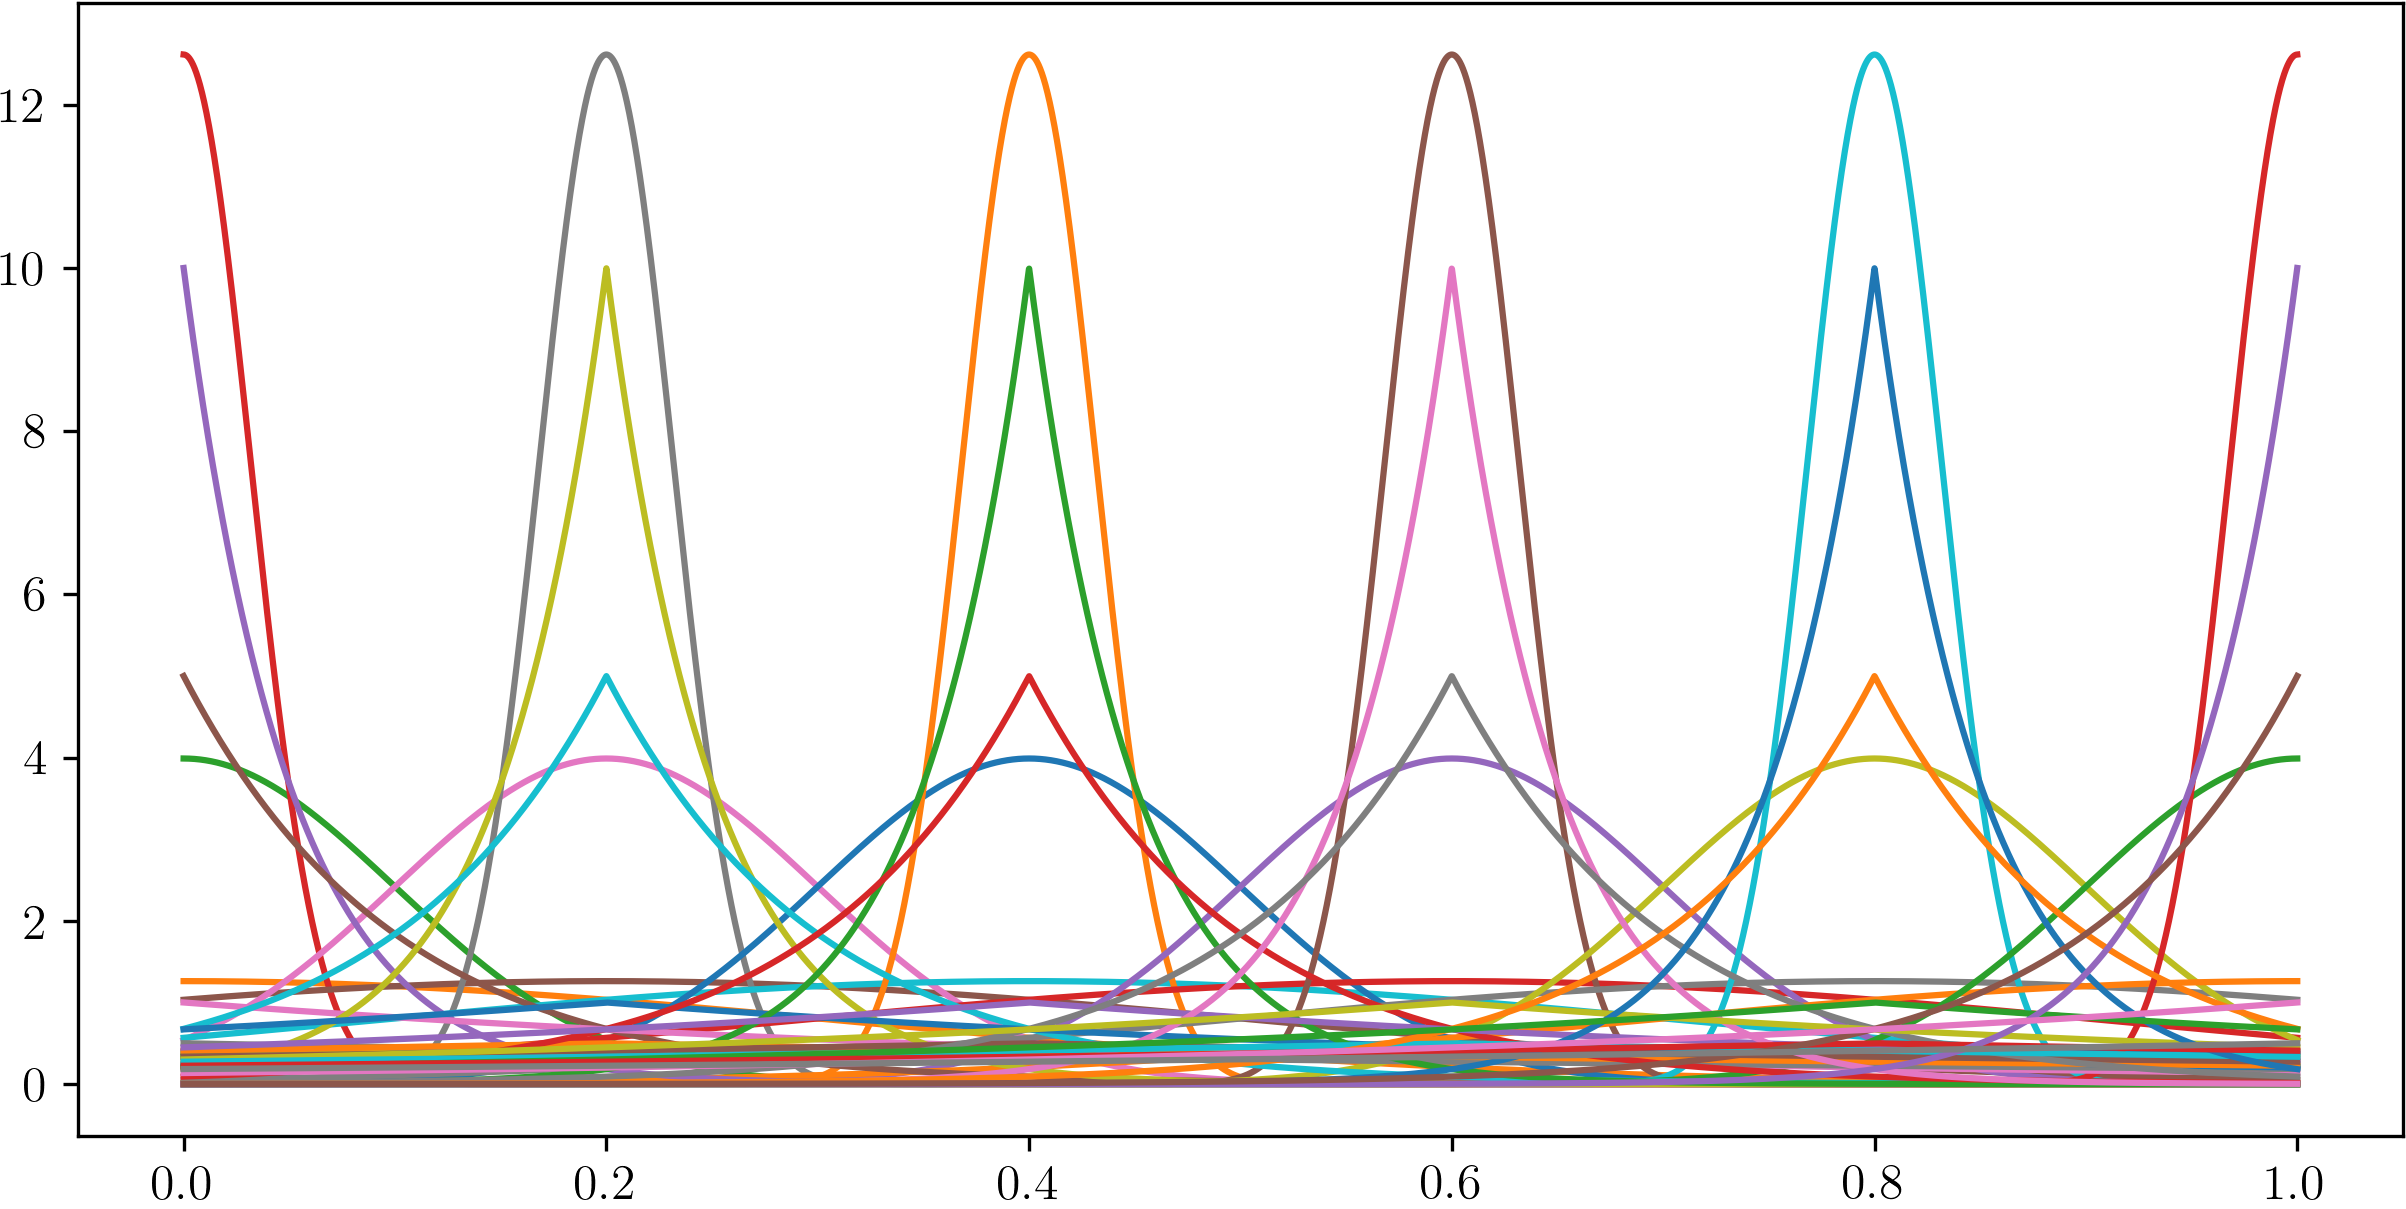
\includegraphics[width=1\textwidth]{TeX_files/lapl_gauss_dict.png}
\caption{$D_{GL}$, union of Gaussians and Laplacians densities.}
\end{figure}
%\item Union of Fourier and Haar aud Gaussians ?
\item The union of $D_{GL}$ with the set of $10$ uniform densities on $(i, i+0.1)\, i\in [0, 0.1,\dots,0.9]$, called $D_{GLU}$.
\end{enumerate}

\subsection{Densities considered}
We considered 5 target densities corresponding to 5 different scenarios. The $1^{st}$ and $2^{nd}$ will asses the performance of our method on uniform based densities, the $3^{rd}$ and $4^th$ on dictionary based density. The last one is a complex density made from elements which are not in the dictionary that we will consider.
\begin{enumerate}
\item{$f_{\textnormal{unif}}$:} A uniform density on $[0,1]$.
\item{$f_{\textnormal{rect}}$:} A mixture of uniform densities on subintervals. This density is called "Rectangular"
\begin{equation}
    f_{\textnormal{rect}}(x)=\frac{10}{7}\b1_{[0,1/5]}+\frac{5}{7}\b1_{[1/5,2/5]}+
    \frac{10}{7}\b1_{[2/5,3/5]}+\frac{10}{7}\b1_{[4/5,1]}
\end{equation}
\item{$f_{\textnormal{gauss}}$:} A mixture of 5 Gaussian densities taken from the dictionary $D_{GL}$ equally centered in $[0,1]$ with same variance.
\begin{equation}
    f_{\textnormal{gauss}}(x)=\sum_{k=1}^5 0.2f_{k}(x) \quad \text{with}\quad f_k=\varphi_{(k/5,0.001)}
\end{equation}

\item{$f_{\textnormal{gauss-lapl}}$:} A mixture of 5 Gaussian and Laplacian densities taken from the dictionary $D_{GL}$ with different variances and scales.
%(multivariate_normal(0.2, 10**(-3)))
%(multivariate_normal(0.6, 10**(-3)))
%(multivariate_normal(0, 10**(-2)))
%(laplace(0.4,0.2))
%(laplace(0.8,0.1))
\begin{equation}
\begin{array}{ll}
f_{\textnormal{gauss-lapl}}(x)=0.2\big(&\varphi_{(0 ,10^{-2})} + \varphi_{(0.2,10^{-3})}+\varphi_{(0.6,10^{-3})}\\
    &+\text{\small Lapl}_{(0.4,0.2)}+\text{\small Lapl}_{(0.8,0.1)} \big)
\end{array}
\end{equation}
\item{$f_{\textnormal{ext}}$:} A mixture of Gaussian and Laplacian densities taken from another dictionary $D_{out}$.
%append(multivariate_normal(0.1, 5*10**(-3)))
%append(multivariate_normal(0.65, 10**(-3)))
%append(multivariate_normal(0.9, 10**(-2)))
%append(laplace(0.5, 0.08))
%append(laplace(0.2, 0.07))
%append(laplace(0.75, 0.05))

\begin{equation}
    f_{\textnormal{ext}}(x)=\sum_{k=1}^7 \frac{1}{7}f_{k}(x) \quad \text{with}\quad f_k\in D_{out}
\end{equation}
\end{enumerate}
These target densities are plotted in \cref{fig:target_densities}.
\begin{figure}[h]
\center
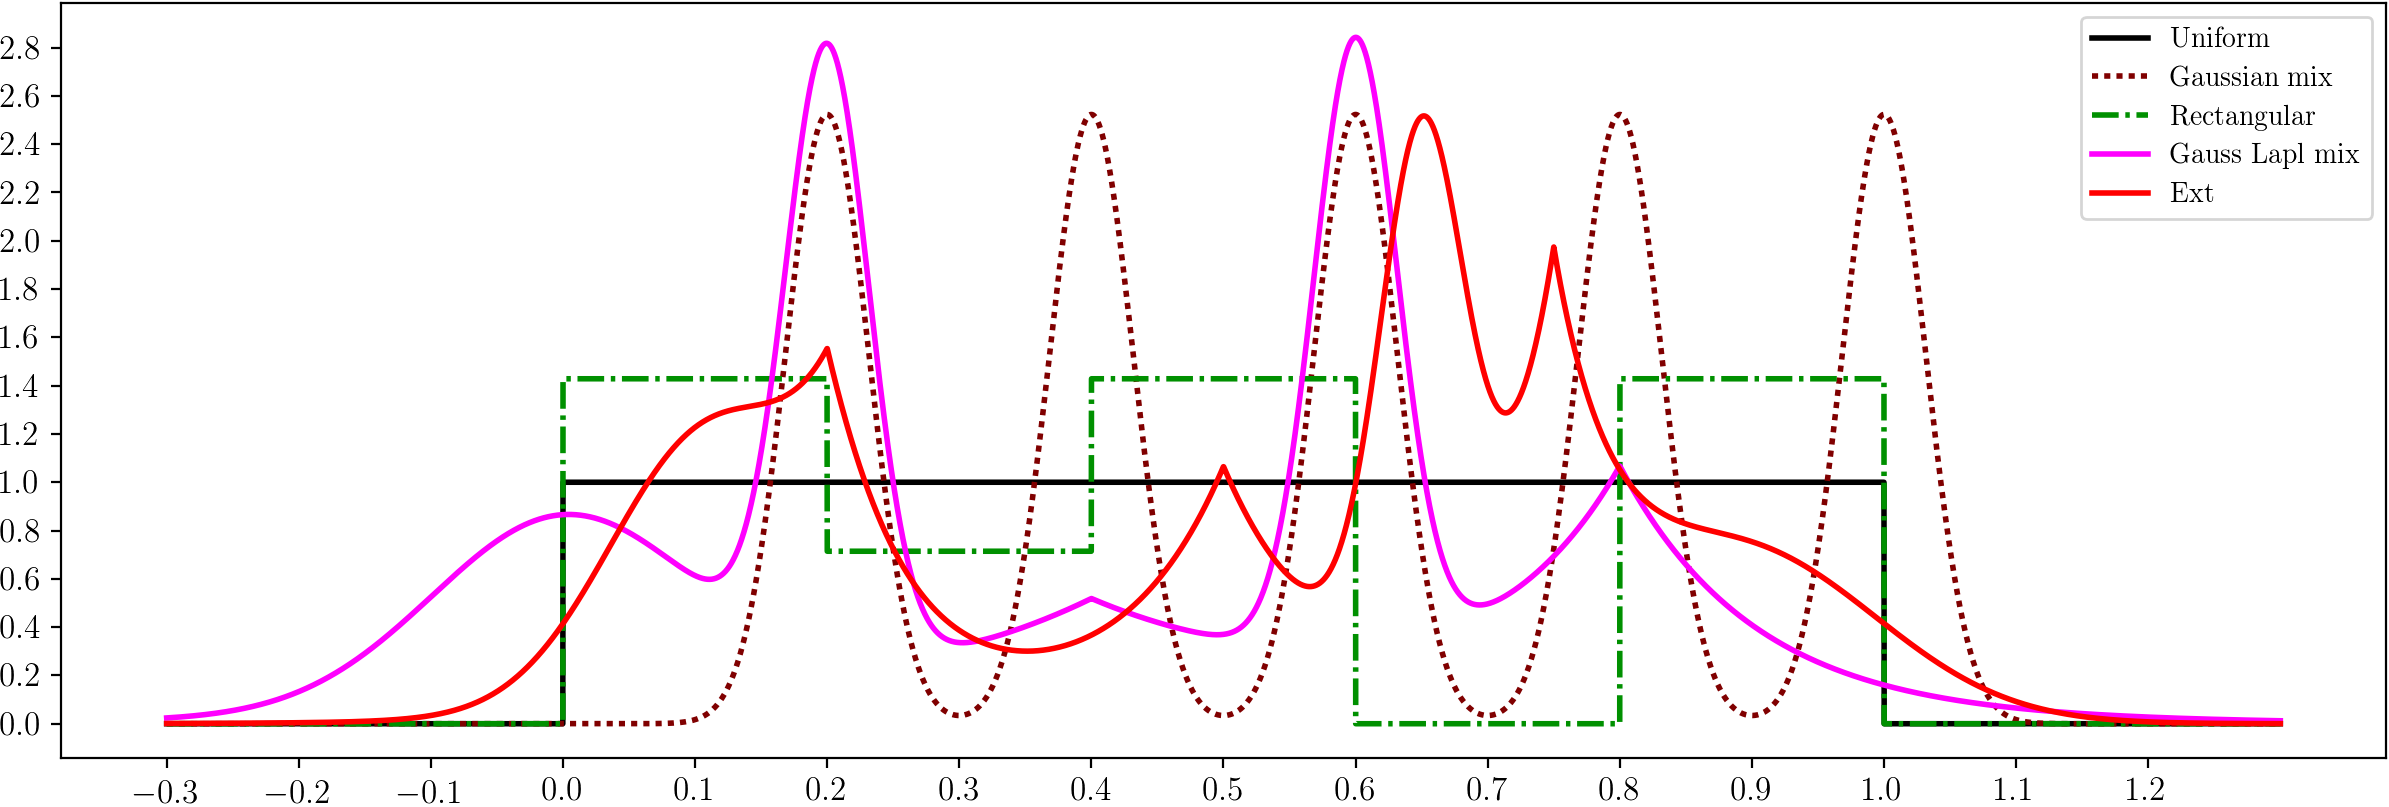
\includegraphics[width=1.1\textwidth]{TeX_files/densities_f_star.png}
\caption{Five target densities considered.}
\label{fig:target_densities}
\end{figure}

\subsection{Discussion of the results}
The dictionaries used for the Adaptive Dantzig and the Maximum likelihood density estimator are $D_{GL}$ and $D_{GLU}$. Note that it is interesting to compare the MLE to A.D as both methods relies on a dictionary. We also benchmarked our method with the Gaussian kernel density estimator, the EM algorithm on Gaussian mixtures model with a model selection by the BIC criterion and Kernel Density Estimators. KDE refers to the kernel density estimate with Scott's rule as chosen by default in the Python library Scipy, KDE-SJ refers to the KDE with the Sheather-Jones bandwidth selector and KDE CV refers to the KDE with bandwidth selected via cross-validation. For each scenario of target density, $f_{\textnormal{unif}}$, $f_{\textnormal{rect}}$, $f_{\textnormal{gauss}}$, $f_{\textnormal{gauss-lapl}}$, $f_{\textnormal{ext}}$ and for each sample size $N$  with $N\in\{100, 500, 1000\}$, we ran 200 simulations. At a first glance, the performance of the MLE seems good in Kullback-Leibler and $L_2$ loss. The method showing the worst performance in all scenarios is the Adaptive Dantzig.

\subsubsection{Studying the bias of the estimator with the densities $f_{\textnormal{unif}}$, $f_{\textnormal{rect}}$ and $f_{\textnormal{ext}}$ on $D_{GL}$}
The densities $f_{\textnormal{unif}}$, $f_{\textnormal{rect}}$ and $f_{\textnormal{ext}}$ were not built with elements in the dictionary $D_{GL}$. Therefore, we can expect that the most dominant term in the error will be the bias term. An interesting observation is the small impact of the size of the sample for the MLE. If we look at $N=100$, the MLE performance is almost as good as KDE-SJ and KDE-CV on the uniform case (\cref{fig:res_uniform_KL_GL}, \cref{fig:res_uniform_L2_GL}). This is surprising since the dictionary given could not provide a good mixture density that approach well this target density. Note that the KDE performs better than KDE-SJ in this scenario only. However, the rectangular density scenario, $f_{\textnormal{rect}}$, shows the worst performance for the MLE (\cref{fig:res_rect_KL_GL}, \cref{fig:res_rect_L2_GL}). It is possible to increase its performance by adding uniform densities on different segments of $[0,1]$ in the dictionary as we will see in \cref{dict_dglu_sect}. Finally, MLE performs poorly in the $f_{\textnormal{ext}}$ scenario, we wanted to measure the performance of dictionary based methods against a complex target density which is not a mixture of elements of the dictionary, see (\cref{fig:res_ext_KL_GL}, \cref{fig:res_ext_L2_GL}). Increasing the size of the sample does not improve the error of the MLE, in this case the choice of the dictionary is clearly crucial. Note that EM-BIC is the best algorithm with $N=100$ but similarly to the MLE, it does not present a significant change as $N$ increase. In these three scenarios, the MLE presents a relative small variance.
%Uniform
\begin{figure}
\center
    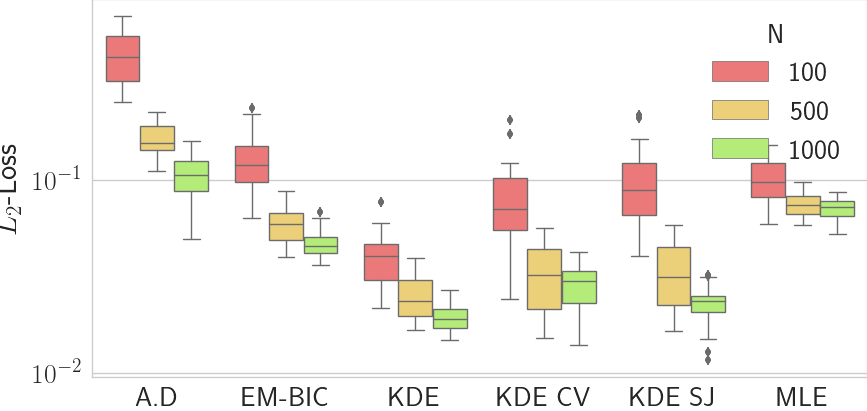
\includegraphics[width=0.8\textwidth]{./TeX_files/res_uniform_L2_GL.png}
    \caption{Results with $f_{\textnormal{unif}}$ in $L2$ loss with $D_{GL}$}
    \label{fig:res_uniform_L2_GL}
\end{figure}

\begin{figure}
\center
    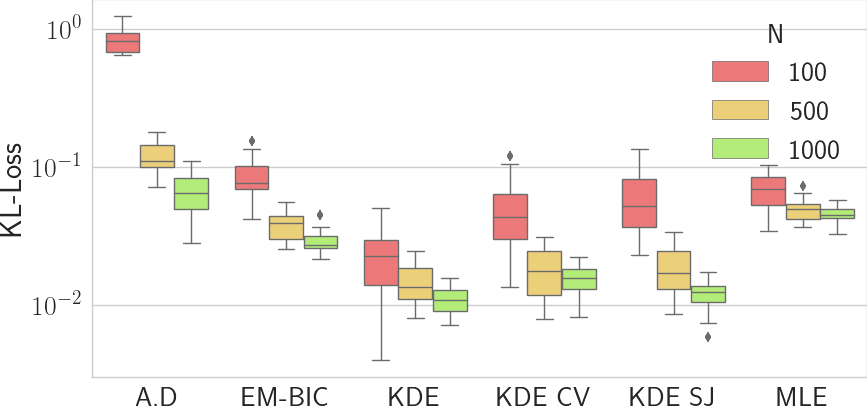
\includegraphics[width=0.8\textwidth]{./TeX_files/res_uniform_KL_GL.png}
    \caption{Results with $f_{\textnormal{unif}}$ in KL loss with $D_{GL}$}
    \label{fig:res_uniform_KL_GL}
\end{figure}
%rect
\begin{figure}
\center
    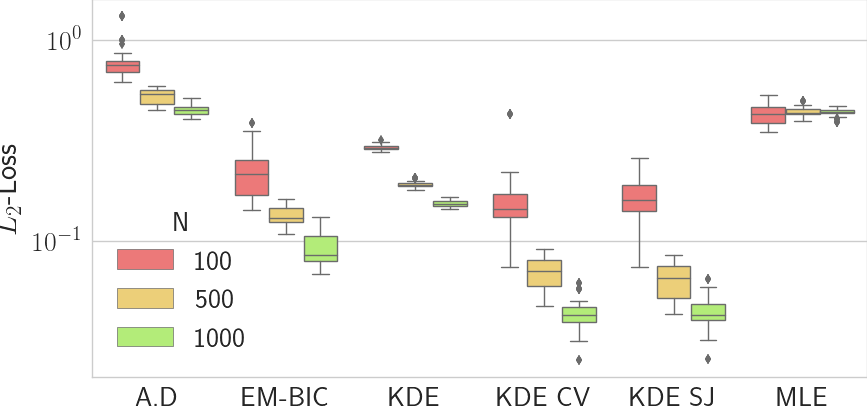
\includegraphics[width=0.8\textwidth]{./TeX_files/res_rect_L2_GL.png}
    \caption{Results with $f_{\textnormal{rect}}$ in $L2$ loss with $D_{GL}$}
    \label{fig:res_rect_L2_GL}
\end{figure}

\begin{figure}
\center
    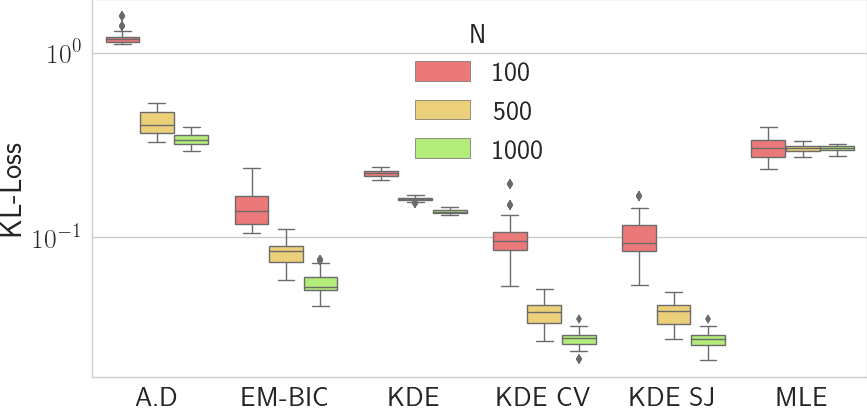
\includegraphics[width=0.8\textwidth]{./TeX_files/res_rect_KL_GL.png}
    \caption{Results with $f_{\textnormal{rect}}$ in KL loss with $D_{GL}$}
    \label{fig:res_rect_KL_GL}
\end{figure}   
%ext
\begin{figure}
\center
    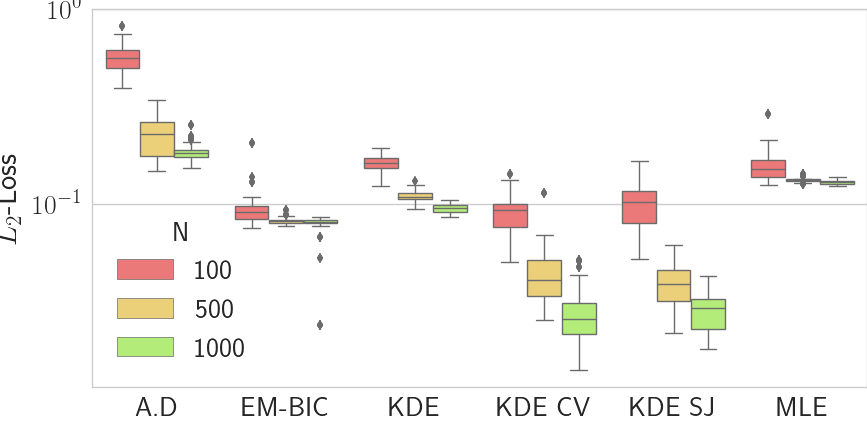
\includegraphics[width=0.8\textwidth]{./TeX_files/res_lapl_gauss_not_dict_L2_GL.png}
    \caption{Results with $f_{\textnormal{ext}}$ in $L2$ loss with $D_{GL}$}
    \label{fig:res_ext_L2_GL}
\end{figure}

\begin{figure}
\center
    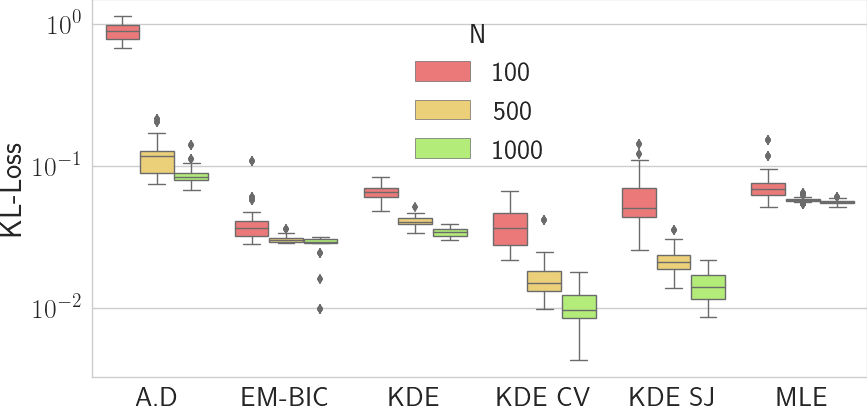
\includegraphics[width=0.8\textwidth]{./TeX_files/res_lapl_gauss_not_dict_KL_GL.png}
    \caption{Results with $f_{\textnormal{ext}}$ in KL loss with $D_{GL}$}
    \label{fig:res_ext_KL_GL}
\end{figure}
\subsubsection{Studying the variance of the estimator with the densities $f_{\textnormal{gauss}}$ and $f_{gauss-lapl}$}
When the target density is the mixture of Gaussians $f_{\textnormal{gauss}}$, the MLE presents the best result, both in $L_2$ and KL loss (\cref{fig:res_gauss_KL_GL}, \cref{fig:res_gauss_L2_GL}). The second best is EM-BIC. Note that the default KDE in Scipy\citep{scipy} with Scott's rule presents the worse result in this scenario which should have reasonably performed well considering the use of Gaussian kernels. This observation should come to mind of the practitioner when applying kernel density estimators with default package setting. The second scenario, $f_{\textnormal{gauss-lapl}}$ is a more complex density made from elements of the dictionary $D_{GL}$ and the MLE is the best method (\cref{fig:res_lapl_gauss_KL_GL}, \cref{fig:res_lapl_gauss_L2_GL}). \sout{Surprisingly the $L_2$ and KL loss of KDE are not similar.}
%gauss
\begin{figure}
\center
    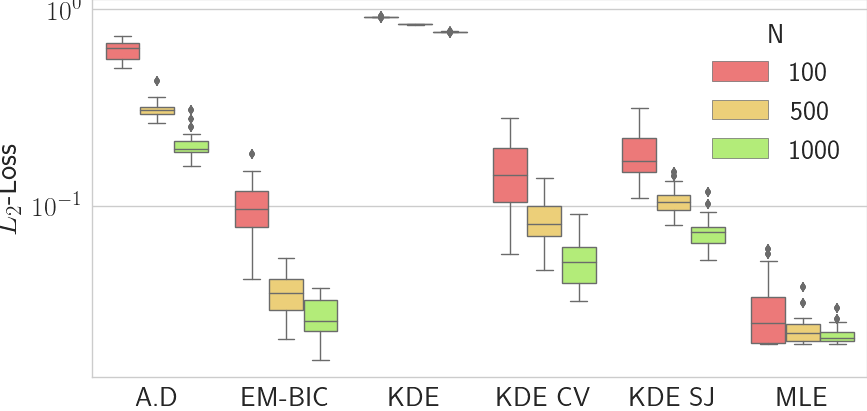
\includegraphics[width=0.8\textwidth]{./TeX_files/res_gauss_L2_GL.png}
    \caption{Results with $f_{\textnormal{gauss}}$ in $L2$ loss with $D_{GL}$}
    \label{fig:res_gauss_L2_GL}
\end{figure}

\begin{figure}
\center
    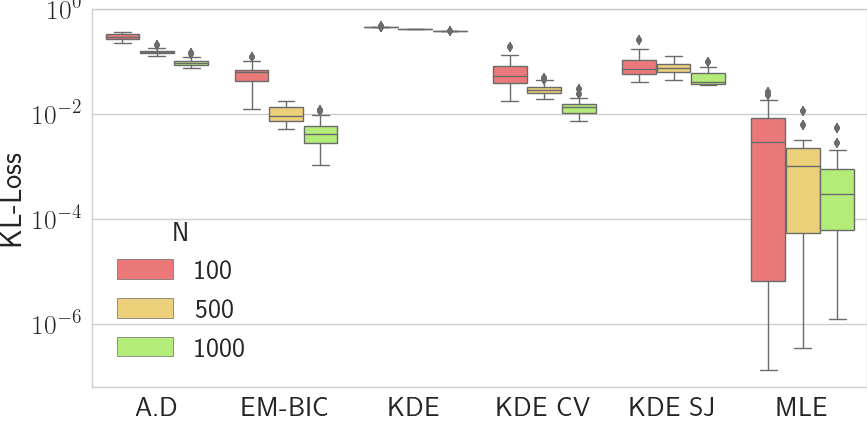
\includegraphics[width=0.8\textwidth]{./TeX_files/res_gauss_KL_GL.png}
    \caption{Results with $f_{\textnormal{gauss}}$ in KL loss with $D_{GL}$}
    \label{fig:res_gauss_KL_GL}
\end{figure}   

%lapl_gauss
\begin{figure}
\center
    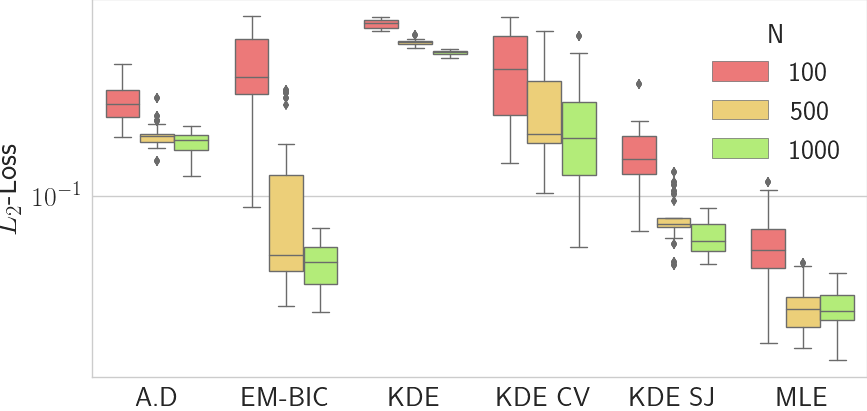
\includegraphics[width=0.8\textwidth]{./TeX_files/res_lapl_gauss_L2_GL.png}
    \caption{Results with $f_{\textnormal{gauss-lapl}}$ in $L2$ loss with $D_{GL}$}
    \label{fig:res_lapl_gauss_L2_GL}
\end{figure}

\begin{figure}
\center
    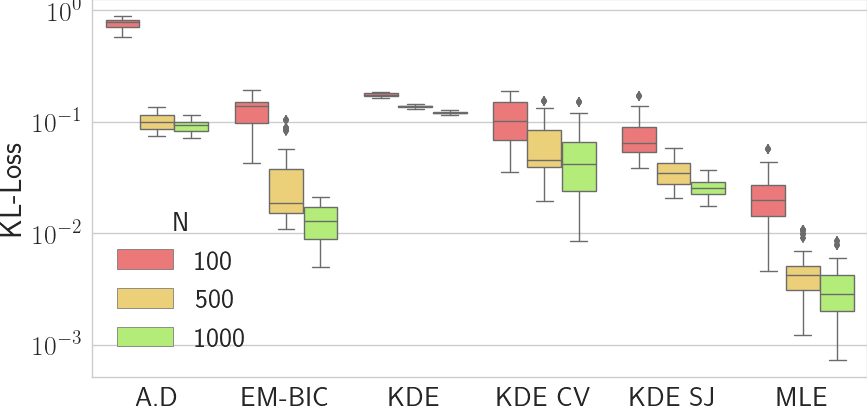
\includegraphics[width=0.8\textwidth]{./TeX_files/res_lapl_gauss_KL_GL.png}
    \caption{Results with $f_{\textnormal{gauss-lapl}}$ in KL loss with $D_{GL}$}
    \label{fig:res_lapl_gauss_KL_GL}
\end{figure}
\subsubsection{The importance of the choice of the dictionary, using $D_{GLU}$. \label{dict_dglu_sect}}
At the sight of the poor performance of the MLE in the uniform and rectangular case, we wanted to add $10$ uniform densities on $(0,0.1),\dots,(0.9,1)$ to the dictionary $D_{GL}$ and study the behavior of our algorithm with this extended dictionary. The results in uniform case are plotted in \cref{fig:res_uniform_L2_GLU} and \cref{fig:res_uniform_KL_GLU}. In rectangular case in \cref{fig:res_rect_KL_GLU} and \cref{fig:res_rect_L2_GLU}. We can see a better performance of the MLE as the size increases. When the size is greater than $500$, our algorithm presents the best performance which in the case of $D_{GLU}$ is not surprising since the MLE possess uniform densities in its dictionary. However, surprisingly the Adaptive Dantzig still presents the worse result. The performance improvement is more visible in the rectangular case. In the case of $f_{\textnormal{gauss}}$ plotted in \cref{fig:res_gauss_L2_GLU} and \cref{fig:res_gauss_KL_GLU}, $f_{gauss-lapl}$ plotted in \cref{fig:res_lapl_gauss_L2_GLU} and \cref{fig:res_lapl_gauss_KL_GLU} and $f_{\textnormal{rect}}$ plotted in \cref{fig:res_ext_L2_GLU} and \cref{fig:res_ext_KL_GLU}, we have no sensible change compared to the dictionary $D_{GL}$.
\begin{figure}
\center
    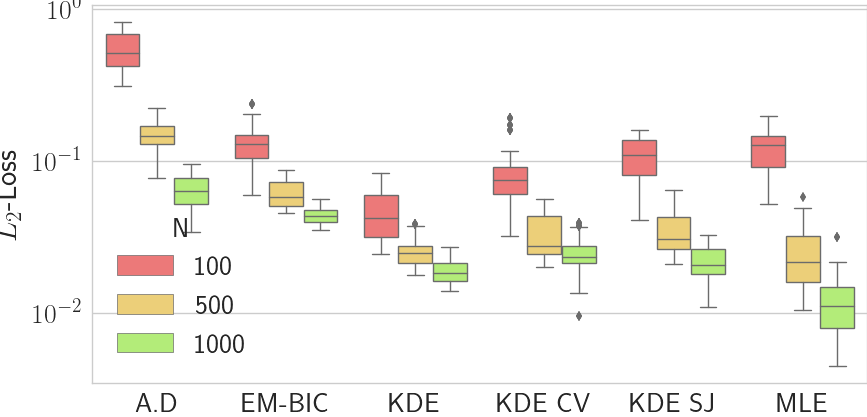
\includegraphics[width=0.8\textwidth]{./TeX_files/res_uniform_L2_GLU.png}
    \caption{Results with $f_{\textnormal{unif}}$ in $L2$ loss with $D_{GLU}$}
    \label{fig:res_uniform_L2_GLU}
\end{figure}

\begin{figure}
\center
    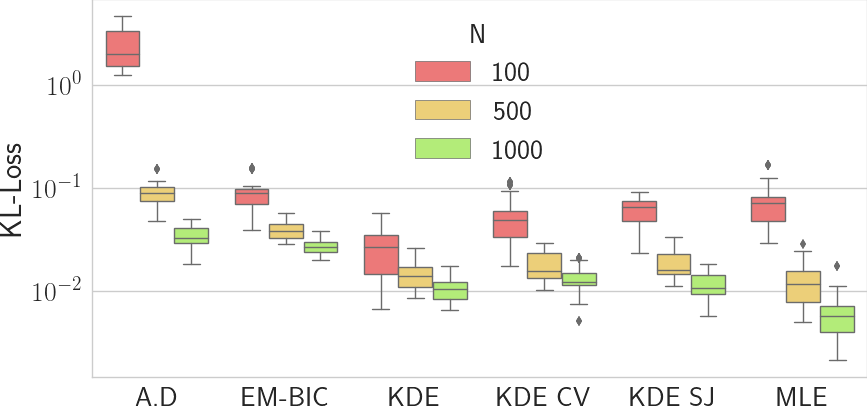
\includegraphics[width=0.8\textwidth]{./TeX_files/res_uniform_KL_GLU.png}
    \caption{Results with $f_{\textnormal{unif}}$ in KL loss with $D_{GLU}$}
    \label{fig:res_uniform_KL_GLU}
\end{figure}
%rect
\begin{figure}
\center
    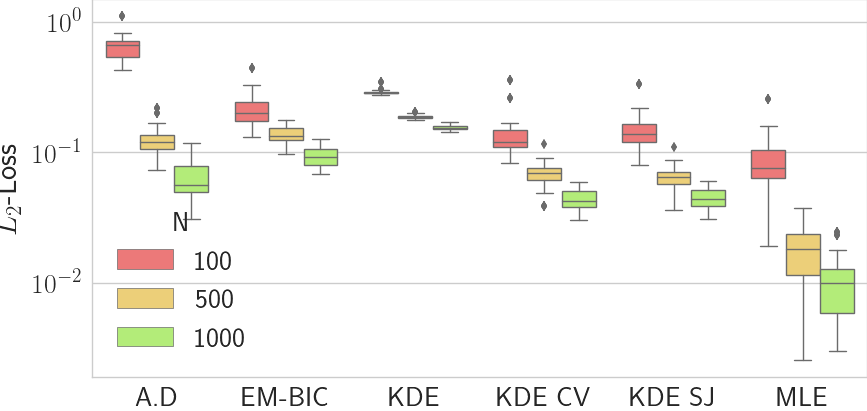
\includegraphics[width=0.8\textwidth]{./TeX_files/res_rect_L2_GLU.png}
    \caption{Results with $f_{\textnormal{rect}}$ in $L2$ loss with $D_{GLU}$}
    \label{fig:res_rect_L2_GLU}
\end{figure}

\begin{figure}
\center
    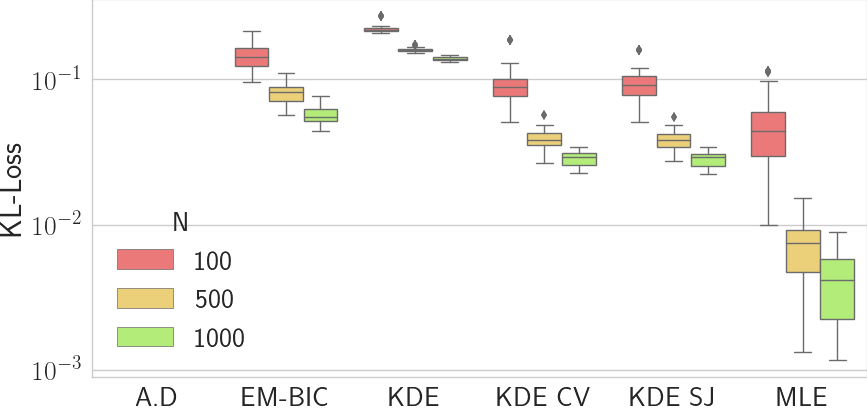
\includegraphics[width=0.8\textwidth]{./TeX_files/res_rect_KL_GLU.png}
    \caption{Results with $f_{\textnormal{rect}}$ in KL loss with $D_{GLU}$}
    \label{fig:res_rect_KL_GLU}
\end{figure}
\begin{figure}
\center
    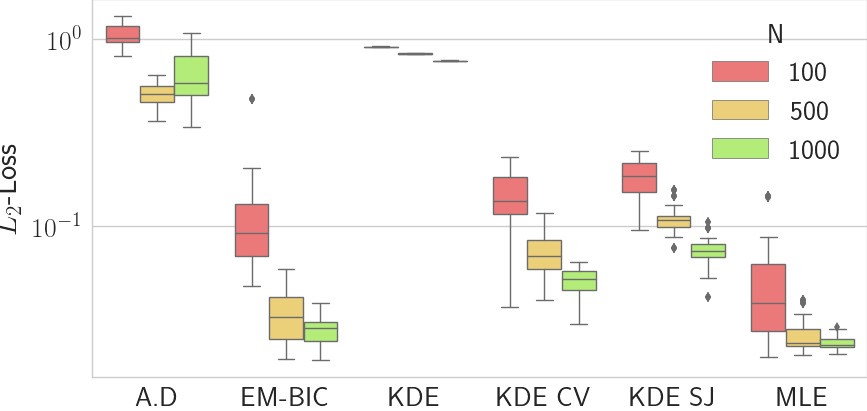
\includegraphics[width=0.8\textwidth]{./TeX_files/res_gauss_L2_GLU.png}
    \caption{Results with $f_{\textnormal{gauss}}$ in $L2$ loss with $D_{GLU}$}
    \label{fig:res_gauss_L2_GLU}
\end{figure}

\begin{figure}
\center
    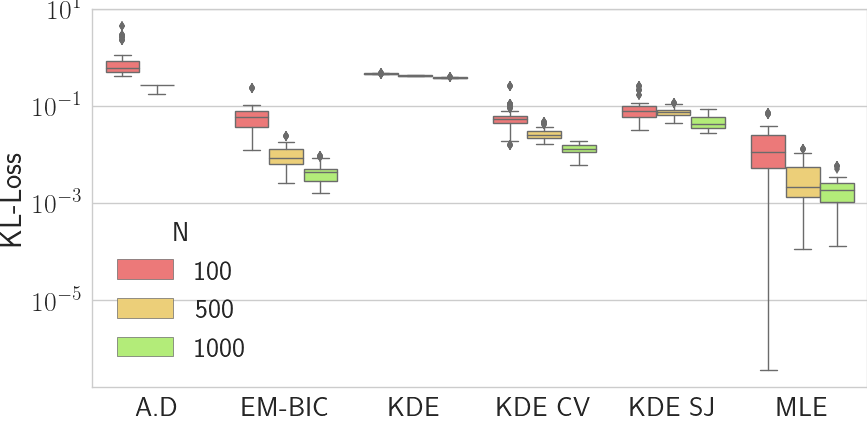
\includegraphics[width=0.8\textwidth]{./TeX_files/res_gauss_KL_GLU.png}
    \caption{Results with $f_{\textnormal{gauss}}$ in KL loss with $D_{GLU}$}
    \label{fig:res_gauss_KL_GLU}
\end{figure}   

%lapl_gauss
\begin{figure}
\center
    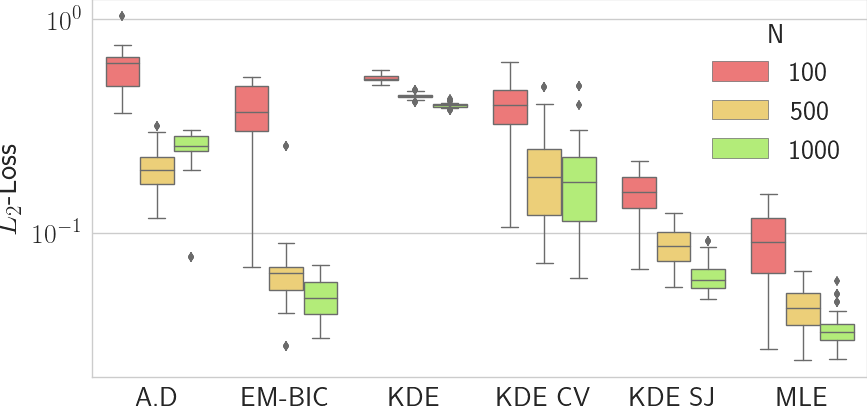
\includegraphics[width=0.8\textwidth]{./TeX_files/res_lapl_gauss_L2_GLU.png}
    \caption{Results with $f_{\textnormal{gauss-lapl}}$ in $L2$ loss with $D_{GLU}$}
    \label{fig:res_lapl_gauss_L2_GLU}
\end{figure}

\begin{figure}
\center
    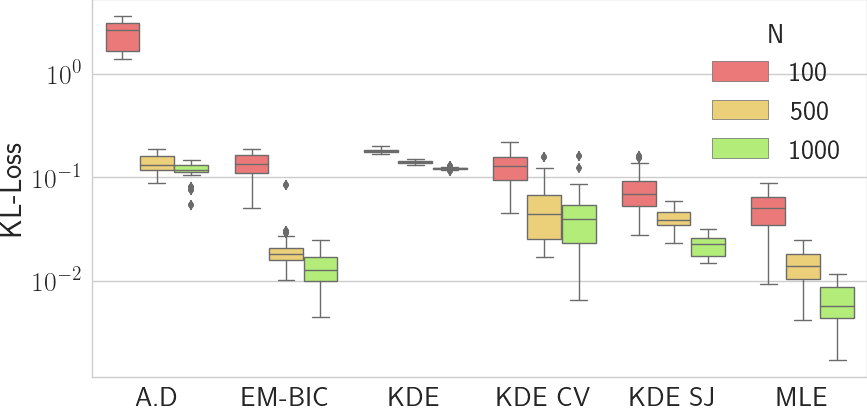
\includegraphics[width=0.8\textwidth]{./TeX_files/res_lapl_gauss_KL_GLU.png}
    \caption{Results with $f_{\textnormal{gauss-lapl}}$ in KL loss with $D_{GLU}$}
    \label{fig:res_lapl_gauss_KL_GLU}
\end{figure}  
%ext
\begin{figure}
\center
    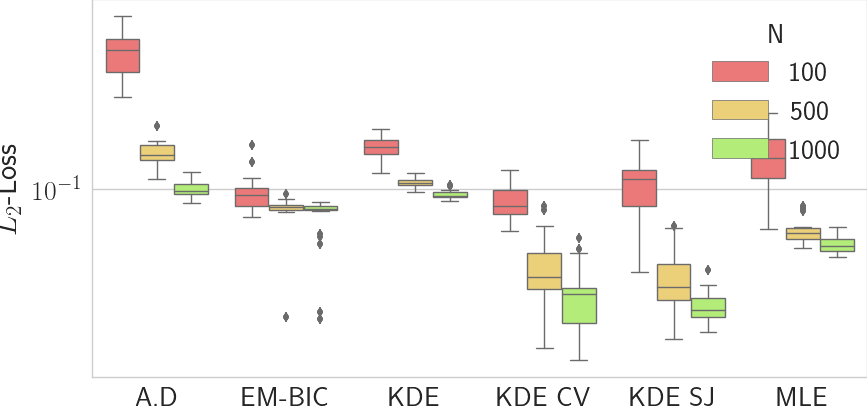
\includegraphics[width=0.8\textwidth]{./TeX_files/res_lapl_gauss_not_dict_L2_GLU.png}
    \caption{Results with $f_{\textnormal{ext}}$ in $L2$ loss with $D_{GLU}$}
    \label{fig:res_ext_L2_GLU}
\end{figure}

\begin{figure}
\center
    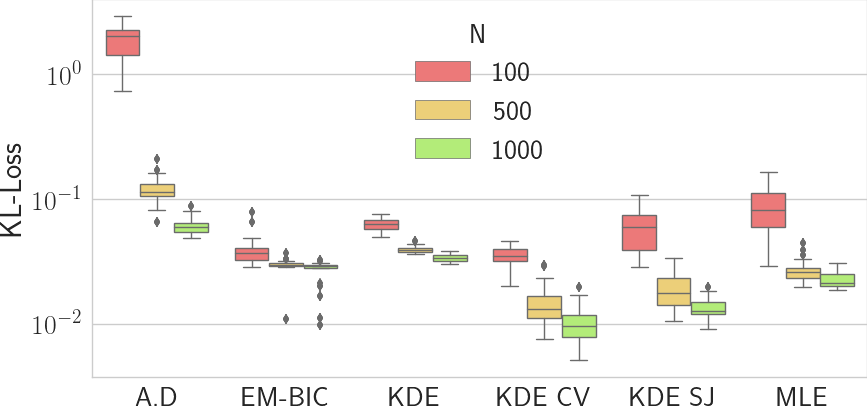
\includegraphics[width=0.8\textwidth]{./TeX_files/res_lapl_gauss_not_dict_KL_GLU.png}
    \caption{Results with $f_{\textnormal{ext}}$ in KL loss with $D_{GLU}$}
    \label{fig:res_ext_KL_GLU}
\end{figure} 
To conclude, the performance of the MLE method in these simulations is promising to achieve a good mixture density estimate. We would like to mention the computational efficiency of the MLE method as it is a convex problem, the whole procedure to construct the estimator is simple and its dimension is the size of the dictionary considered. During our simulations, the MLE method showed interesting time of computation. Our algorithm was coded in Python with some elements accelerated with the Just-In-Time (JIT) compiler Numba \citep{numba}. Compared to compiled optimized versions of KDE and EM from Scipy and Scikit-Learn\citep{scikit-learn}, we are confident that the computation time of our algorithm can be significantly decreased. Another important point is in the case of high dimensional data, KDE and EM+BIC methods are known to present poor performance in this setting. Our method need the computation of the matrix $(f_j(X_i))_{(i,j)\in [N]\times [K]}$ which might consume a lot of memory. Some techniques such as a Mini-batch approach can help. Furthermore, at the light of the results in the uniform and rectangular case, the choice of the dictionary is a cornerstone in constructing a good mixture density. It can not be too large due to memory limitations. This is a classical problem of dictionary-based methods.

\begin{figure}
\center
    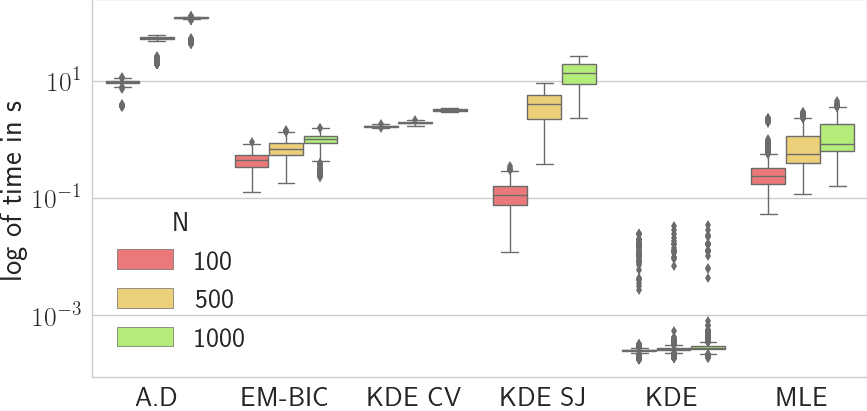
\includegraphics[width=0.8\textwidth]{./TeX_files/res_times.png}
    \caption{Computation times}
    \label{fig:res_times}
\end{figure}

\section{Real use case}

The code is available on github